%%%%%%%%%%%%%%%%%%%%%%%%%%%%%%%%%%%%%%%%%%%%%%%%%%%%%%%%%%%%
%%  This Beamer template was created by Cameron Bracken.
%%  Anyone can freely use or modify it for any purpose
%%  without attribution.
%%
%%  Last Modified: January 9, 2009
%%

\documentclass[xcolor=x11names,compress]{beamer}

%% General document %%%%%%%%%%%%%%%%%%%%%%%%%%%%%%%%%%
\usepackage{graphicx}
\usepackage{tikz}
\usetikzlibrary{arrows}
\usetikzlibrary{decorations.pathmorphing} % wiggly line
\usetikzlibrary{positioning} % relative positioning
\usetikzlibrary{fit} % box fitting
%%%%%%%%%%%%%%%%%%%%%%%%%%%%%%%%%%%%%%%%%%%%%%%%%%%%%%


%% Beamer Layout %%%%%%%%%%%%%%%%%%%%%%%%%%%%%%%%%%
\useoutertheme[subsection=false,shadow]{miniframes}
\useinnertheme{default}
\usefonttheme{serif}
\usepackage{palatino}

\setbeamerfont{title like}{shape=\scshape}
\setbeamerfont{frametitle}{shape=\scshape}

\setbeamercolor*{lower separation line head}{bg=DeepSkyBlue4} 
\setbeamercolor*{normal text}{fg=black,bg=white} 
\setbeamercolor*{alerted text}{fg=red} 
\setbeamercolor*{example text}{fg=black} 
\setbeamercolor*{structure}{fg=black} 
 
\setbeamercolor*{palette tertiary}{fg=black,bg=black!10} 
\setbeamercolor*{palette quaternary}{fg=black,bg=black!10} 

\renewcommand{\(}{\begin{columns}}
\renewcommand{\)}{\end{columns}}
\newcommand{\<}[1]{\begin{column}{#1}}
\renewcommand{\>}{\end{column}}
%%%%%%%%%%%%%%%%%%%%%%%%%%%%%%%%%%%%%%%%%%%%%%%%%%

\usepackage{adjustbox}
\usepackage{amsmath}
\usepackage{stmaryrd}
\usepackage{wasysym}
\usepackage{etoolbox}
\usepackage{separationlogic}
\newcommand{\xspace}{}

\begin{document}


%%%%%%%%%%%%%%%%%%%%%%%%%%%%%%%%%%%%%%%%%%%%%%%%%%%%%%
%%%%%%%%%%%%%%%%%%%%%%%%%%%%%%%%%%%%%%%%%%%%%%%%%%%%%%
\begin{frame}
\title{A Program Logic for Verification of Security Properties in Secure
  ECMAScript}
\author{
  Thomas Wood \\[10pt]
  {\scriptsize
    Supervised by:\\[0pt]
    Dr. Gareth Smith \and Prof. Philippa Gardner
  } 
}
\titlepage
\end{frame}

%%%%%%%%%%%%%%%%%%%%%%%%%%%%%%%%%%%%%%%%%%%%%%%%%%%%%%
%%%%%%%%%%%%%%%%%%%%%%%%%%%%%%%%%%%%%%%%%%%%%%%%%%%%%%
\section{\scshape Background}
\begin{frame}{Secure ECMAScript}
  \begin{itemize}
    \item ECMAScript = JavaScript
    \item Secure ECMAScript (SES) -- language variant supporting \emph{Object
      capability} programming
    \item Key introduction: \emph{restricted evaluation}
  \end{itemize}
\end{frame}

\begin{frame}{Restricted Evaluation Example}
  \begin{center}
    \texttt{reval(\emph{code}, \emph{imports});}
  \end{center}


  \visible<3->{
    \texttt{m = Membrane(\{a:a, b:b\})} \\
  }
  \only<1-2>{
    \texttt{reval(\emph{code}, \{a:a, b:b\});}
  }
  \only<3->{
    \texttt{reval(\emph{code}, m.access)}
  }

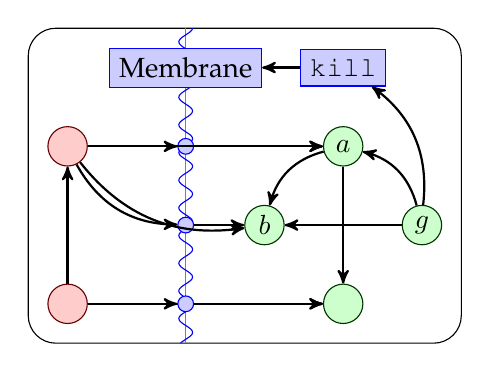
\begin{tikzpicture}[
    object/.style={circle, minimum size=5mm, inner sep=0},
    trusted/.style={object, draw=green!20!black, fill=green!20!white},
    untrusted/.style={object, draw=red!40!black, fill=red!20},
    membranec/.style={draw=blue, fill=blue!20},
    membrane/.style={object, membranec, minimum size=2mm},
    arrow/.style={thick, >=stealth'},
    pre/.style={arrow, <-},
    post/.style={arrow, ->}
  ]
  \draw[clip,rounded corners=10, use as bounding box] (0,0.5) rectangle (5.5,4.5);
  \node[trusted] (a) at (4,3) {$a$};
  \node[trusted] (b) at (3,2) {$b$}
    edge [pre,bend left] (a);
  \node[trusted] (g) at (5,2) {$g$}
    edge [post,bend right] (a)
    edge [post] (b);
  \node[trusted] (c) at (4,1) {}
    edge [pre] (a);

  \visible<1-2>{\draw[help lines] (2,0) -- (2,5);}
  \visible<3-5>{
    \draw[membrane,decorate,decoration=snake,fill=none] (2,0) -- (2,10);
    \node[membranec,rectangle] (membrane) at (2,4) {Membrane};
    \node[membranec,rectangle] (kill) at (4,4) {\texttt{kill}}
      edge [post] (membrane)
      edge[pre,bend left] (g);
    \node[membrane] (ma) at (2,3) {};
    \node[membrane] (mb) at (2,2) {};
  }
  \visible<3-4>{
    \draw [post] (ma) to (a);
    \draw [post] (mb) to (b);
  }

  \node[untrusted] (ua) at (0.5,3) {};
  \node[untrusted] (ub) at (0.5,1) {}
    edge [post] (ua);

  \visible<1-2>{
    \draw [post] (ua) to (a);
    \draw [post,bend right] (ua) to (b);
  }
  \visible<2>{\draw [post] (ub) to (c);}
  \visible<3->{
    \draw [post] (ua) to (ma);
    \draw [post,bend right] (ua) to (mb);
  }
  \visible<4->{
    \node[membrane] (mc) at (2,1) {}
      edge [pre] (ub);
  }
  \visible<4>{
    \draw[post] (mc) to (c);
  }
\end{tikzpicture}
\end{frame}

\begin{frame}{Separation Logic}
  \begin{itemize}
    \item $\sep$ is $\land$ with \emph{disjointness}

      $(x \pointsto 4 \sep y \pointsto 7)$
      
      $h \satisfies P \sep Q \iff \exists h_1,h_2 \st h \equiv h_1 \disju h_2
      \land h_1 \satisfies P \land h_2 \satisfies Q$

    \item $\wand$, \emph{magic wand}, performs heap extension

      $(x \pointsto 5) \wand Q$
  $h \satisfies P \wand Q \iff \forall h' \st (h' \satisfies P) \land h \disj
    h' \impl (h \disju h' \satisfies Q)$
  \end{itemize}
\end{frame}

\begin{frame}{Hoare Logic}
  \begin{itemize}
    \item Fault-avoiding Hoare triple
      
      $\tr{P}{\js{e}}{Q}$

      If \js{e} evaluated in heap satisfying $P$, then evaluation \emph{will not fault},
      and if it terminates, will terminate with heap satisfying $Q$.

    \item Frame Rule

      $
        \staterule{}
        {\tr{P}{C}{Q}}
        {\tr{P \sep R}{C}{Q \sep R}}
        {\mathrm{modifies}(C) \disj \mathrm{free}(R)}
      $

  \end{itemize}
\end{frame}

\section{\scshape Project}
\begin{frame}{Extending Separation Logic}
  \begin{itemize}
    \item \emph{Reintroduce} a global view of heap, $h_g$

    \item Extend standard operators

      {\small$
  h,h_g \satisfies P \sep Q \iff
    \exists h_1,h_2 \st h \equiv h_1 \disju h_2 \land
    (h_1,h_g \satisfies P) \land (h_2,h_g \satisfies Q)
  $}

    \item Define new operators:
      \begin{itemize}
        \item Backpointer, $\bp$

          Asserts what references are permitted to \emph{point to} an object

        \item Hypothesising wand, $\boxwand$

          A variant of $\wand$
    \end{itemize}
  \end{itemize}
\end{frame}

\begin{frame}{Backpointer}
  \begin{center}
    $E_1 \bp E_2$ \\
    $E_1$ may be pointed at by \emph{at most} the locations in set $E_2$
  {\small
\begin{align*}
  h, h_g \satisfies E_1 \bp E_2 \iff &
    \forall (l,x) \in \dom(h_g) \st h_g(l,x) = \evalle{E_1}
    \impl (l,x) \in \evalle{E_2} \land {} \\
    & h \equiv (\evalle{E_1}, @bp) \pointsto \_
\end{align*}
}
  \end{center}

  \begin{itemize}
    \item \emph{Not} pure operator
  \end{itemize}
  
\end{frame}

\begin{frame}{Hypothesising Wand}
  $\wand$ traditionally has \emph{two purposes}, to extend the footprint of an
  assertion with:
  \begin{itemize}
    \item Current heap state
    \item Proposed heap state -- for Weakest Precondition generation
  \end{itemize}
  \ \\[0.5cm]

  Need \emph{two} operators, one for each purpose:
  {\small
$h,h_g \satisfies P \wand Q \iff \forall h' \st (h',h_g \satisfies P) \land h \disj h'
    \land h' \subseteq h_g
  \impl (h \disju h', h_g \satisfies Q) $

  $h,h_g \satisfies P \boxwand Q \iff \forall h' \st (h',h_g[h'] \satisfies P)
  \land h \disj h' \impl (h \disju h', h_g[h'] \satisfies Q)$
  }
\end{frame}

\begin{frame}{New Inference Rules}
  $
  \staterule{(Assign)}
    {
      \tr P {\js{e_1}} {R \sep \rv \doteq \fld{L}{X}} \\
      \tr R {\js{e_2}} {Q \sep (L,X) \pointsto V_3 \sep \rv \doteq V_1} \\
      Q = S \sep \getValue(Ls, V_1, V_2) \sep \ReadWrite(L) \sep
      \bpGen(V_2, L, X, s)
    }
    {\tr P {\js{e_1 = e_2}} {Q \sep (L,X) \pointsto V_2 \sep \rv \doteq V_2}}
  $\\[0.5cm]

  $
    \bpGen(V,L,x,s) \triangleq  V \dotin \loc \sep V \bp \{(L,x)\} \cup s
  $

\end{frame}

\begin{frame}{Membrane Proof -- Predicates}
  {\small
    $\begin{array}{l}
  MembraneInstance(M, F_{MR}, F_K) \\
  \quad \triangleq \obj_M(\js{ref}: \_, @this: \_, @proto: \nil,
      \js{MembraneRef}: F_{MR}, \js{kill}: F_{K}) \sep {} \\
  \quad     \phantom{{} \triangleq {}} \newfun_{F_{MR}}(M:\_, \js{ref}, \lambda_{MR}, \_) \\
  alive(M, F_{MR}, F_K)  \triangleq MembraneInstance(M, F_{MR}, F_K) \sep (M, killed) \pointsto \false \\
  dead(M, F_{MR}, F_K) \triangleq MembraneInstance(M, F_{MR}, F_K) \sep (M,
  killed) \pointsto \true\\
  \\

  \visible<2->{kill(F_K, M) \triangleq \fun_{F_K}(M:\_, \_ , \lambda_K, \_) \\}
  \\
  \visible<3->{
  MRef_{MR}(M,r,F_A,S,T) \triangleq \fun_{F_A}(MR:M:\_, \js{field}, \lambda_A, \_) \sep {} \\
         \phantom{{} \triangleq {}} \fullobj_{MR}(\js{ref}: r, \js{access}: F_A, @this: \_, @proto: \nil) \sep
    r \bp S \cup T
  }\\
\\
\visible<4->{
  MRset_M([], \{(M, \js{ref})\}) \triangleq \lemp \\
  MRset_M(L:Ls, Ts') \triangleq MRset_M(Ls, Ts) \sep Ts' \doteq Ts \cup \{(L, \js{ref})\}
}
\end{array}$
}
\end{frame}

\begin{frame}{Membrane Proof -- Specification}
  Membrane construction:\\[0.2cm]

  \begin{adjustbox}{width=\textwidth,keepaspectratio}
  $
  \begin{array}{l}
    \logic{
      (\_, \js{ref}) \pointsto ref \sep
      ref \bp S \sep
      ref \dotin \loc \sep
      \ls \doteq Ls
    } \\
    \js{Membrane(ref);} \\
    \logic{
      (\_, ref) \pointsto ref \sep
      ref \dotin \loc \sep
      \ls \doteq Ls \sep {} \\
      \exists M, F_K, F_A, F_{MR}, MR, L \st \args{
        alive(M, F_{MR}, F_K) \sep
        kill(F_K,M) \sep
        MRef_{MR}(M, ref, F_A, S, T) \sep {} \\
        MRset([MR],T) \sep
        \fullobj_L(\js{access}:F_A,\js{kill}:F_K) \sep
        \rv \doteq L
      }
    }
  \end{array}
  $
\end{adjustbox}\\[0.5cm]

  Membrane revocation:\\[0.2cm]
  \begin{adjustbox}{width=\textwidth,keepaspectratio}
  $
  \begin{array}{l}
    \logic{
      (\_,\js{kill}) \pointsto F_K \sep kill(F_K,M) \sep (dead(M, F_{MR}, F_K)
      \lor alive(M, F_{MR}, F_K))
    } \\
    \js{kill();} \\
    \logic{
      (\_,\js{kill}) \pointsto F_K \sep kill(F_K,M) \sep dead(M, F_{MR}, F_K)
    } \\
  \end{array}
  $
\end{adjustbox}
\end{frame}

\begin{frame}{Membrane Proof -- Specification}
  Access method:\\[0.2cm]
  \begin{adjustbox}{width=\textwidth,keepaspectratio}
$
  \begin{array}{l}
    \logic{
      (\_,\js{access}) \pointsto F_{A_1} \sep
      alive(M, F_{MR}, F_K) \sep
      MRef_{R_1}(M,ref,F_{A_1},S_1,T_1) \sep
      MRset(Ls,T_1) \sep {} \\

      (\_, \js{field}) \pointsto F \sep F \dotin \uvars \sep
      \getValue(\_, \fld{ref}{F}, V) \sep
      V \dotin \loc \sep
      V \bp S_2
    } \\
    \js{access(field);} \\
    \logic{
      (\_, \js{access}) \pointsto F_{A_1} \sep
      alive(M, F_{MR}, F_K) \sep
      MRef_{R_1}(M,ref,F_{A_1},S_1,T_2) \sep {} \\
      \exists R_2, F_{A_2} \st \args{
        MRset(R_2:Ls,T_2) \sep
        MRef_{R_2}(M,V,F_{A_2},S_2,T_2) \sep
        \rv \doteq F_{A_2}
      } \sep {} \\
      (\_, \js{field}) \pointsto F \sep F \dotin \uvars \sep
      \getValue(\_, \fld{ref}{F}, V) \sep
      V \dotin \loc
    }
  \end{array}
$
\end{adjustbox}
\end{frame}

\begin{frame}{Conclusions}
\begin{itemize}
  \item Specified the semantics of the SES language
  \item Program logic for SES
  \item First use of separation logic to reason about object capability security
  \item Proofs for some object capability programs
  \item Discovered duality of uses for magic wand operator
  \item Confirmed logic matches intuitions of a programmer in the field
\end{itemize}
\end{frame}

\end{document}

